\documentclass{article}
\usepackage[utf8]{inputenc}
\usepackage{graphicx}
\usepackage{listings}
\title{Information System - Lab work 8}
\author{Tran Thi Hong Hanh}
\date{10 November 2017}

\begin{document}

\maketitle
\section*{Database}

\begin{figure}[h]
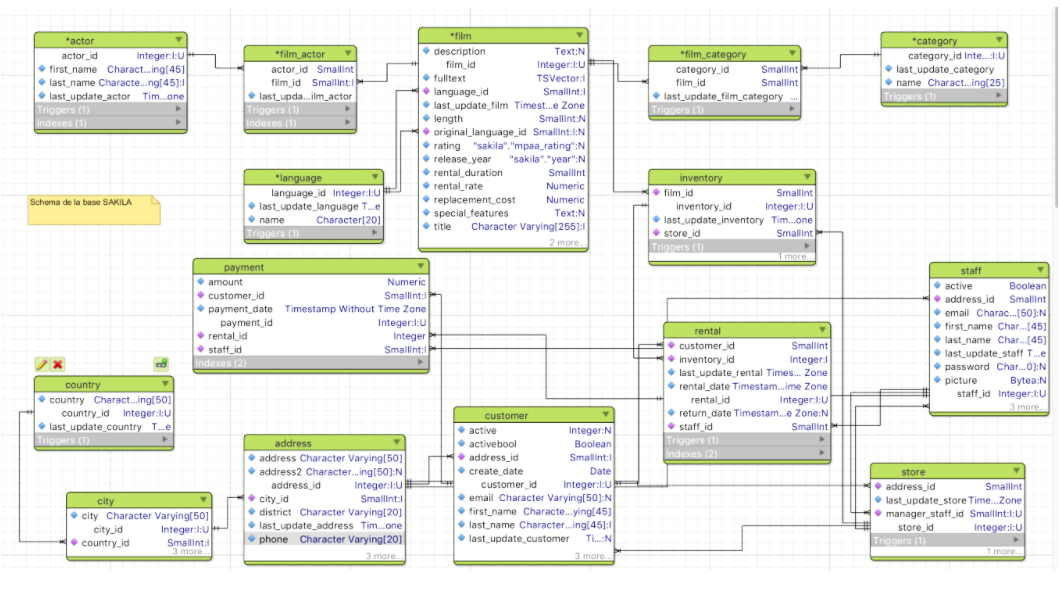
\includegraphics[scale = 0.6]{schema.PNG}
\caption{Visual example of Sakila database schema}
\end{figure}

\section*{SQL queries}
\begin{enumerate}
	\item List names of all the languages in the database (sorted alphabetically)?\\
	\begin{lstlisting}{showstringspaces=false}[language=SQL]
SELECT * FROM language
ORDER BY name ASC;
	\end{lstlisting}
	
	\item List full names of actors with "GER" in their last name, ordered by their first name.\\
	\begin{lstlisting}{showstringspaces=false}
SELECT CONCAT(first_name," ",last_name) AS full_name
FROM actor
WHERE last_name LIKE "%GER%"
ORDER BY first_name ASC;
	\end{lstlisting}
	
	\item Find all the addresses where postal code starts with "57", and return addresses sorted.
	\begin{lstlisting}{showstringspaces=false}
SELECT *
FROM address
WHERE postal_code LIKE "57%"
ORDER BY address;
	\end{lstlisting}
	
	\item How many films involve a "DRAWRF" in their titles?
	
	\begin{lstlisting}{showstringspaces=false}
SELECT COUNT(*) 
FROM film
WHERE title LIKE "%DRAWF%";
	\end{lstlisting}
	
	\item Find full names of actors who played in a film involving 'WAR' in title and longer than 2.5 hours, along with the title, run length and release year of the movie, sorted by the actors' last names. 
	
	\begin{lstlisting}{showstringspaces=false}

	\end{lstlisting}

	\item Find all the film categories in which there are between 55 and 65 films. Return the names of these categories and the number of films per category, sorted by the number of films descending.
	
	\begin{lstlisting}{showstringspaces=false}

	\end{lstlisting}

	\item In how many film categories is the average difference between the film replacement cost and the rental rate larger than 17?
	
	\begin{lstlisting}{showstringspaces=false}

	\end{lstlisting}

	\item Find the address district(s) name(s) such that the minimal postal code in the district(s) is maximal over all the districts. Make sure your query ignores empty postal codes and district names.
	
	\begin{lstlisting}{showstringspaces=false}

	\end{lstlisting}
		
	\item Find the names (first and last) of all the actors and customers whose first name is the same as the first name of the actor with ID 101 (exclude the actor with ID 101).
	
	\begin{lstlisting}{showstringspaces=false}

	\end{lstlisting}
			
\end{enumerate}

\section*{Results}

The figure below presents the results after implement queries (limit from 0 to 10 for some long results
) above:\\
\begin{figure}
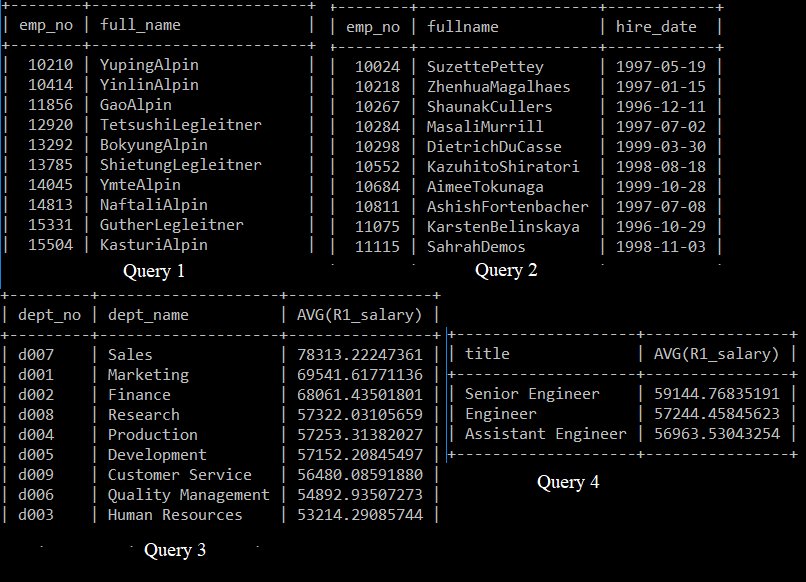
\includegraphics[scale = 0.9]{result.PNG}
\caption{Results}
\end{figure}
\end{document}
